\PassOptionsToPackage{quiet}{fontspec}
\documentclass[12pt,a4paper,UTF8]{article}
\usepackage{thesis} % 格式控制
\usepackage{indentfirst}
\usepackage{float}
\usepackage{xcolor}

\setlength{\parindent}{2em} % 控制首行缩进  
\addtolength{\parskip}{3pt} % 控制段落距离  
\onehalfspacing % 1.5倍行距  
\graphicspath{{./figures/}} % 指定图片所在文件夹  


\classname{Signal and System}  % 设置课程名称
\makepagestyle{}{\printclassname ~Lab Report}




\begin{document}
\maketitlepage{Lab2}{西2-310}{Zhixuan Zheng}{3230103913}{\today}{Xiaoming Chen} % Cover page

\maketoc    %目录页
\section{Problem1}
\subsection{Problem}
\begin{figure}[H]
  \centering
  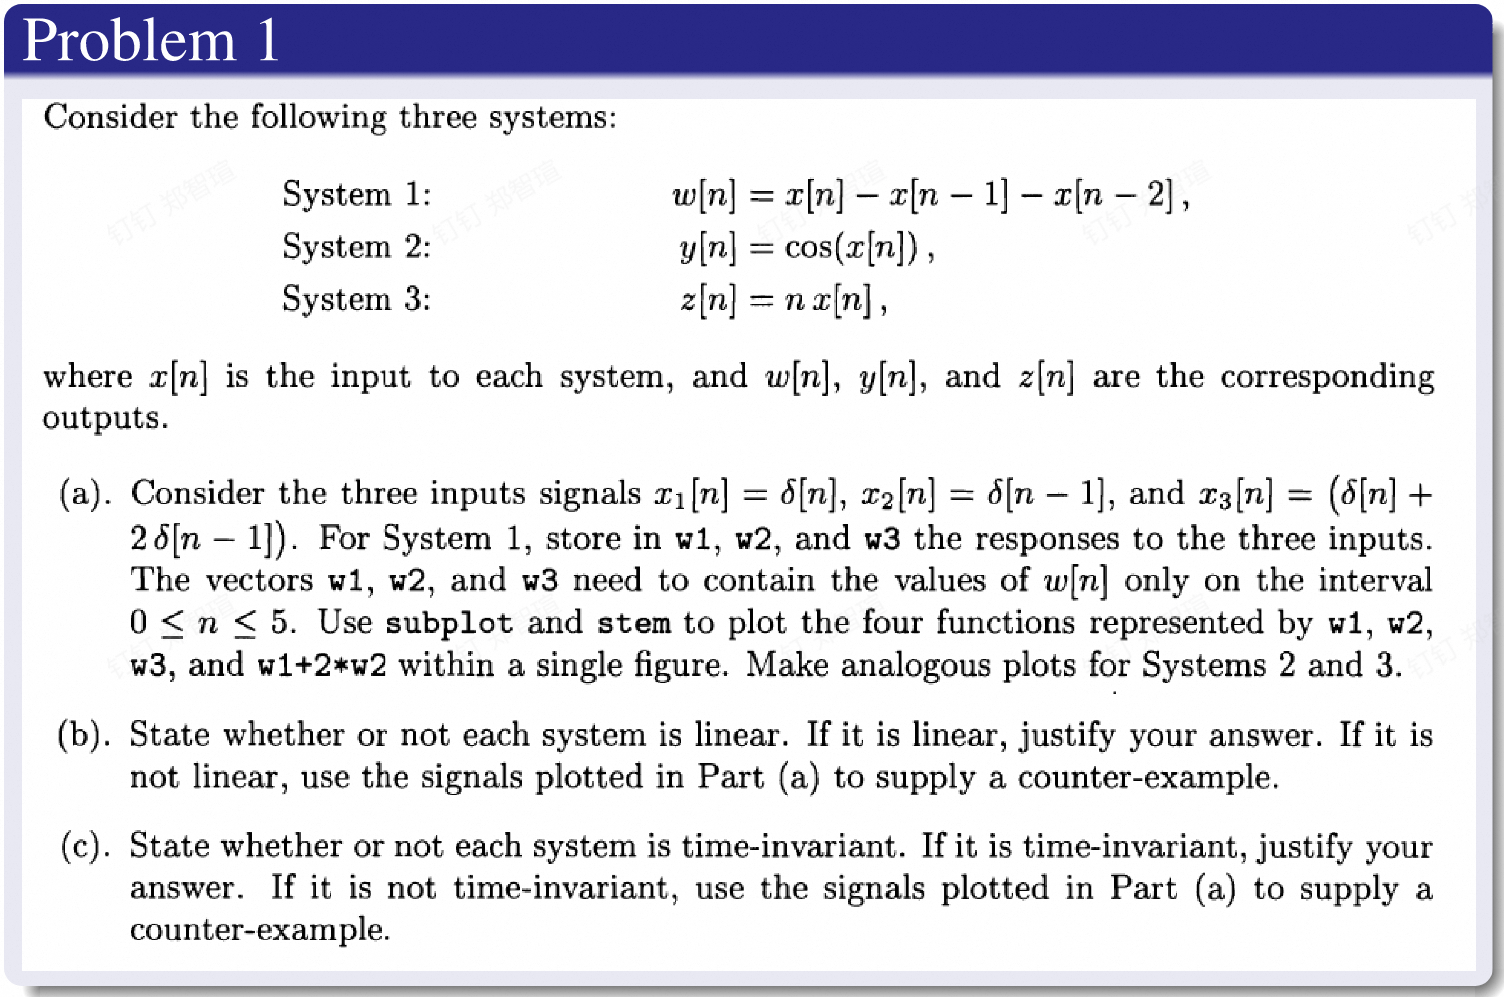
\includegraphics[width=0.75\linewidth]{figures/P1.png} % 数字表示放缩比例
  \caption{Problem1} % 图片标题
\end{figure}
\subsection{Answer}
\begin{figure}[H]
  \centering
  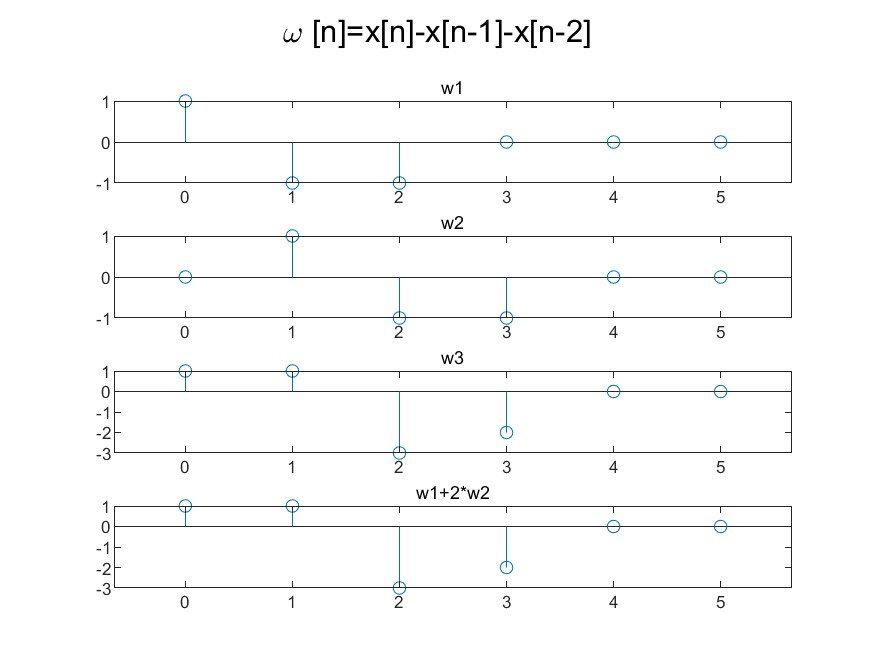
\includegraphics[width=0.75\linewidth]{figures/A1a1.jpg} % 数字表示放缩比例
  \caption{Answer1} % 图片标题
\end{figure}
\begin{figure}[H]
  \centering
  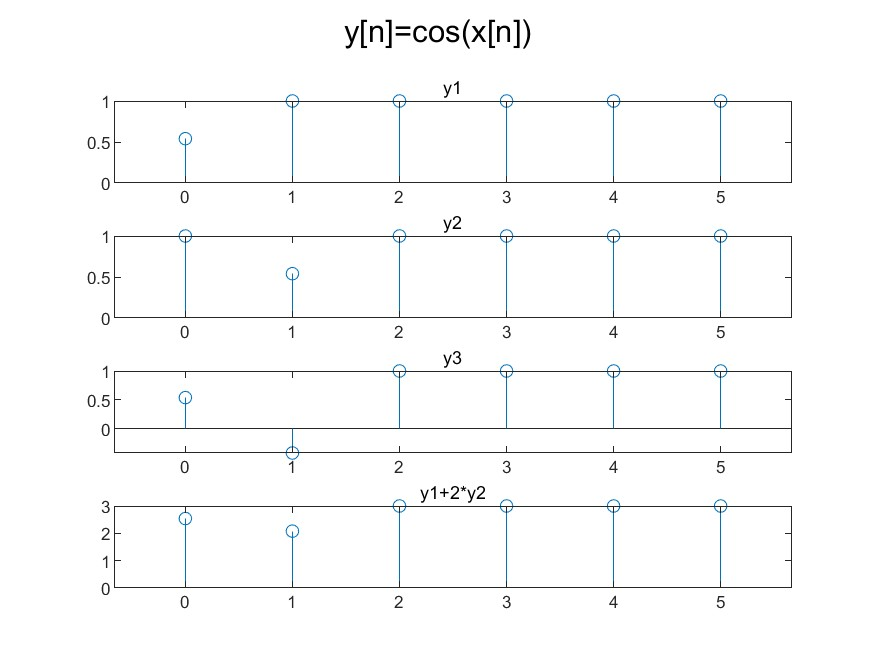
\includegraphics[width=0.75\linewidth]{figures/A1a2.jpg} % 数字表示放缩比例
  \caption{Answer1} % 图片标题
\end{figure}
\begin{figure}[H]
  \centering
  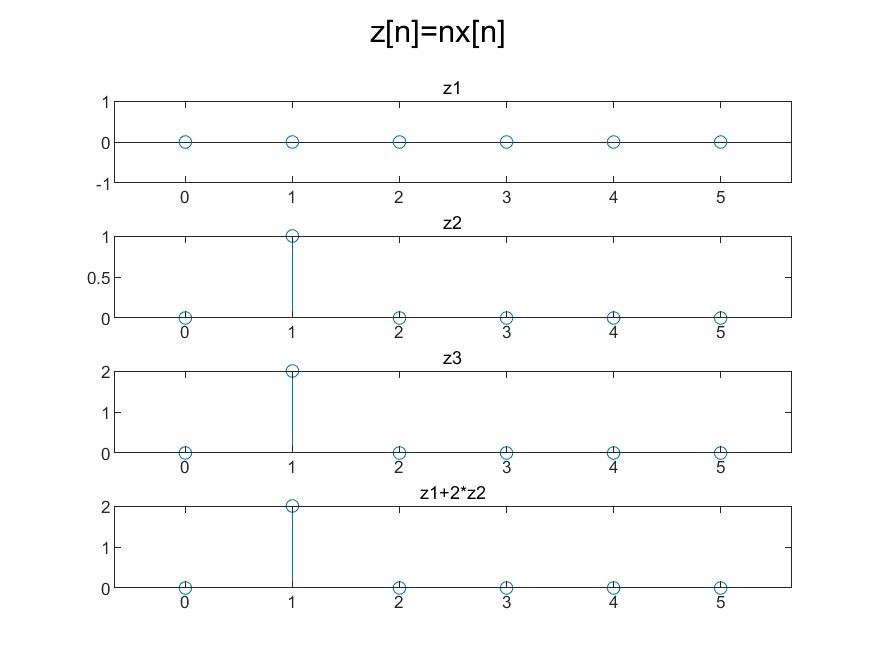
\includegraphics[width=0.75\linewidth]{figures/A1a3.jpg} % 数字表示放缩比例
  \caption{Answer1} % 图片标题
\end{figure}

\subsubsection*{(b) Linearity Analysis}  
A system is \textbf{linear} if it satisfies both \textbf{additivity} and \textbf{homogeneity}. That is, for any inputs \( x_1[n] \), \( x_2[n] \), and scalars \( a \), \( b \):  
\[
T\{a x_1[n] + b x_2[n]\} = a T\{x_1[n]\} + b T\{x_2[n]\}
\]

\textbf{System 1:} \( w[n] = x[n] - x[n-1] - x[n-2] \)  
\begin{itemize}
    \item \textbf{Homogeneity:}  
    If the input is scaled by \( a \), i.e., \( x[n] \to a x[n] \), then  
    \[
    w[n] = a x[n] - a x[n-1] - a x[n-2] = a \left( x[n] - x[n-1] - x[n-2] \right)
    \]  
    The output is also scaled by \( a \). Therefore, the system satisfies homogeneity.

    \item \textbf{Additivity:}  
    For two inputs \( x_1[n] \) and \( x_2[n] \), the outputs are:  
    \[
    w_1[n] = x_1[n] - x_1[n-1] - x_1[n-2]
    \]  
    \[
    w_2[n] = x_2[n] - x_2[n-1] - x_2[n-2]
    \]  
    If the input is \( x_1[n] + x_2[n] \), then  
    \[
    w[n] = (x_1[n] + x_2[n]) - (x_1[n-1] + x_2[n-1]) - (x_1[n-2] + x_2[n-2])
    \]  
    \[
    = w_1[n] + w_2[n]
    \]  
    The system satisfies additivity.
\end{itemize}  
\textbf{Conclusion:} System 1 satisfies both additivity and homogeneity, so it is \textbf{linear}.

\vspace{0.5em}

\textbf{System 2:} \( y[n] = \cos(x[n]) \)  
\begin{itemize}
    \item \textbf{Homogeneity:}  
    If the input is scaled by \( a \),  
    \[
    y[n] = \cos(a x[n])
    \]  
    In general,  
    \[
    \cos(a x[n])c a \cos(x[n])
    \]  
    so the system does not satisfy homogeneity.

    \item \textbf{Additivity:}  
    For two inputs \( x_1[n] \) and \( x_2[n] \),  
    \[
    y_1[n] = \cos(x_1[n]), \quad y_2[n] = \cos(x_2[n])
    \]  
    If the input is \( x_1[n] + x_2[n] \),  
    \[
    y[n] = \cos(x_1[n] + x_2[n]) \neq \cos(x_1[n]) + \cos(x_2[n])
    \]  
    so the system does not satisfy additivity.
\end{itemize} 
\textcolor{red}{Also,in Figure3,we can see that $y_3 \neq y_1+2*y_2$.} 

\textbf{Conclusion:} System 2 fails both additivity and homogeneity, so it is \textbf{nonlinear}. \\
\vspace{0.5em}

\textbf{System 3:} \( z[n] = n x[n] \)  
\begin{itemize}
    \item \textbf{Homogeneity:}  
    If the input is scaled by \( a \),  
    \[
    z[n] = n (a x[n]) = a (n x[n])
    \]  
    so the system satisfies homogeneity.

    \item \textbf{Additivity:}  
    For two inputs \( x_1[n] \) and \( x_2[n] \),  
    \[
    z_1[n] = n x_1[n], \quad z_2[n] = n x_2[n]
    \]  
    If the input is \( x_1[n] + x_2[n] \),  
    \[
    z[n] = n (x_1[n] + x_2[n]) = n x_1[n] + n x_2[n] = z_1[n] + z_2[n]
    \]  
    so the system satisfies additivity.
\end{itemize}  
\textbf{Conclusion:} System 3 satisfies both additivity and homogeneity, so it is \textbf{linear}.

\vspace{1em}

\subsubsection*{(c) Time-Invariance Analysis}  
A system is \textbf{time-invariant} if shifting the input by \( k \) results in an identical shift in the output:  
\[
T\{x[n-k]\} = y[n-k]
\]

\vspace{0.5em}

\textbf{System 1:} \( w[n] = x[n] - x[n-1] - x[n-2] \)  
\begin{itemize}
    \item Shift the input by \( k \):  
    \[
    x[n] \to x[n - k]
    \]  
    The output becomes  
    \[
    w[n] = x[n - k] - x[n - k - 1] - x[n - k - 2]
    \]  
    This is equivalent to  
    \[
    w[n - k] = x[(n - k)] - x[(n - k) - 1] - x[(n - k) - 2]
    \]  
    so the system is time-invariant.
\end{itemize}  
\textbf{Conclusion:} System 1 is \textbf{time-invariant}.

\vspace{0.5em}

\textbf{System 2:} \( y[n] = \cos(x[n]) \)  
\begin{itemize}
    \item Shift the input by \( k \):  
    \[
    x[n] \to x[n - k]
    \]  
    The output becomes  
    \[
    y[n] = \cos(x[n - k])
    \]  
    This is equivalent to  
    \[
    y[n - k] = \cos(x[(n - k)])
    \]  
    so the system is time-invariant.
\end{itemize}  
\textbf{Conclusion:} System 2 is \textbf{time-invariant}.

\vspace{0.5em}

\textbf{System 3:} \( z[n] = n x[n] \)  
\begin{itemize}
    \item Shift the input by \( k \):  
    \[
    x[n] \to x[n - k]
    \]  
    The output becomes  
    \[
    z[n] = n \cdot x[n - k]
    \]  
    The expected time-invariant output should be  
    \[
    z[n - k] = (n - k) \cdot x[n - k]
    \]  
    but  
    \[
    n x[n - k] \neq (n - k) x[n - k]
    \]  
    so the system is time-variant.
\end{itemize}  
\textcolor{red}{Additionally, in Figure 4, we can see that 
$z_1$ shifted 1 unit to the right is not equal to $z_2$.} 
\textbf{Conclusion:} System 3 is \textbf{time-variant}.

\vspace{1em}

\subsubsection*{Final Summary}

\begin{center}
\begin{tabular}{|c|c|c|}
\hline
\textbf{System} & \textbf{Linearity} & \textbf{Time-Invariance} \\
\hline
System 1 & Linear & Time-Invariant \\
System 2 & Nonlinear & Time-Invariant \\
System 3 & Linear & Time-Variant \\
\hline
\end{tabular}
\end{center}

\clearpage

\section{Problem2a,2b}
\subsection{Problem}
\begin{figure}[H]
  \centering
  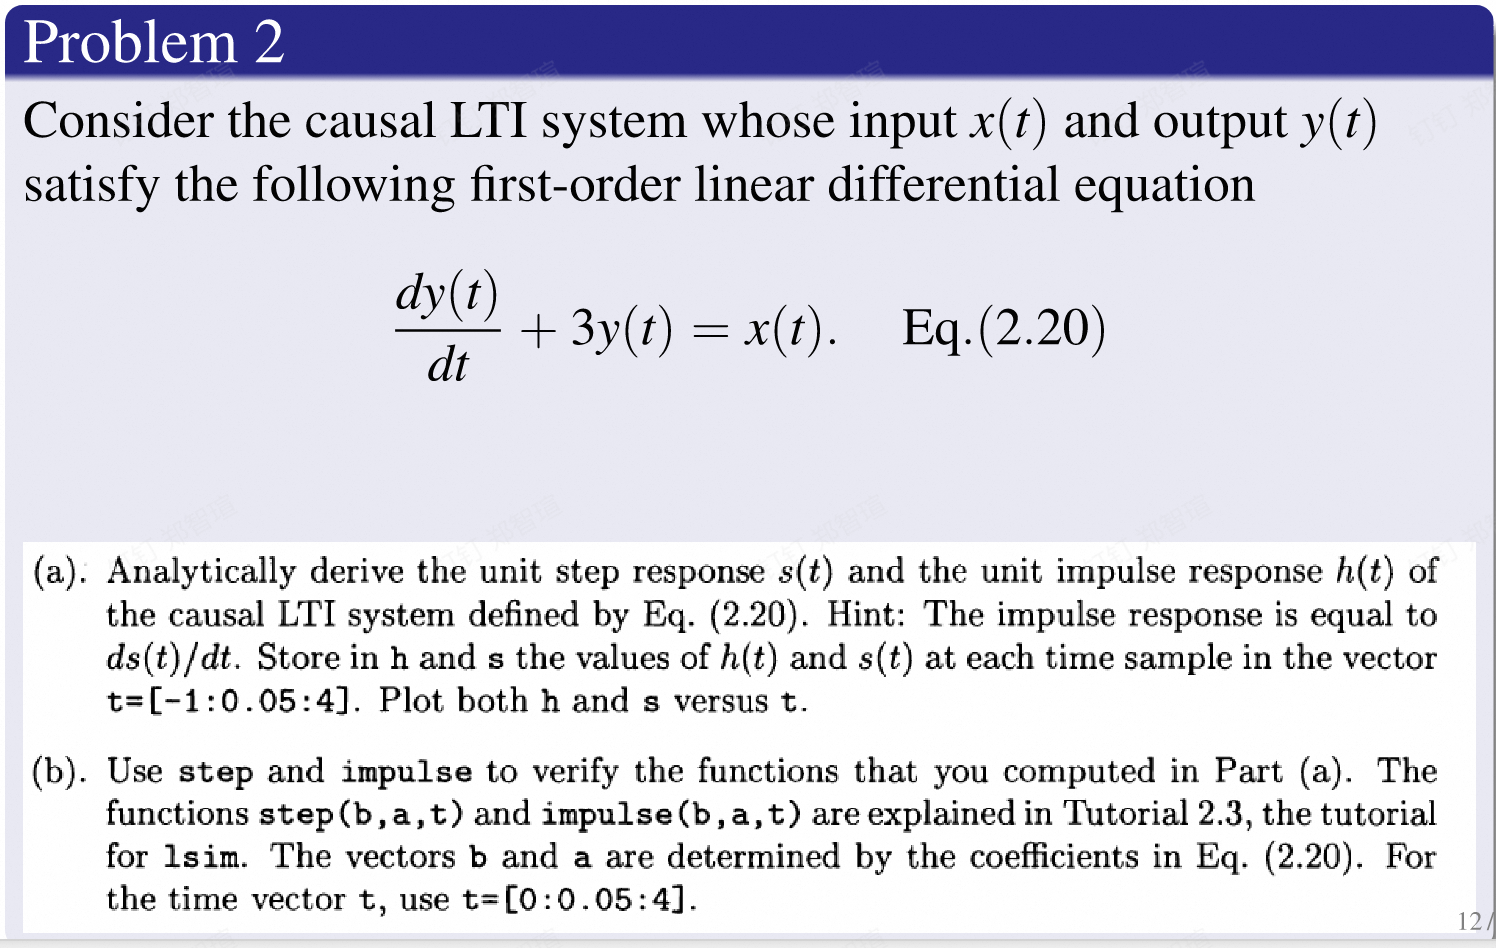
\includegraphics[width=0.75\linewidth]{figures/P21.png} % 数字表示放缩比例
  \caption{Problem2a,2b} % 图片标题
\end{figure}

\subsection{Answer}
\subsubsection*{(a) Analytical Derivation of the Step Response $s(t)$ and Impulse Response $h(t)$}

Consider the causal LTI system defined by the differential equation:
\[
\frac{dy(t)}{dt} + 3y(t) = x(t) \qquad \text{Eq. (2.20)}
\]

\textbf{Step 1: Laplace Transform of the Equation}

Taking the Laplace Transform of both sides of the differential equation (assuming zero initial conditions, i.e., $y(0^{-}) = 0$):
\[
s \cdot Y(s) + 3Y(s) = X(s)
\]
Factor out $Y(s)$:
\[
Y(s) \left( s + 3 \right) = X(s)
\]
Thus, the transfer function $H(s)$ is:
\[
H(s) = \frac{Y(s)}{X(s)} = \frac{1}{s + 3}
\]

\textbf{Step 2: Impulse Response $h(t)$}

The impulse response $h(t)$ is the inverse Laplace Transform of $H(s)$:
\[
h(t) = \mathcal{L}^{-1} \left\{ \frac{1}{s + 3} \right\}
\]
We have:
\[
h(t) = e^{-3t} u(t)
\]
where $u(t)$ is the unit step function.

\textbf{Step 3: Step Response $s(t)$}

The step response $s(t)$ is the system's response to a unit step input $x(t) = u(t)$.

In the Laplace domain, the input is:
\[
X(s) = \frac{1}{s}
\]
Then the output is:
\[
S(s) = H(s) \cdot X(s) = \frac{1}{s + 3} \cdot \frac{1}{s} = \frac{1}{s(s + 3)}
\]

Perform partial fraction decomposition:
\[
\frac{1}{s(s + 3)} = \frac{A}{s} + \frac{B}{s + 3}
\]
Multiply both sides by $s(s + 3)$:
\[
1 = A(s + 3) + B(s)
\]

Solving for $A$ and $B$:
\begin{itemize}
    \item Let $s = 0$: $1 = A(0 + 3) \Rightarrow A = \frac{1}{3}$
    \item Let $s = -3$: $1 = B(-3) \Rightarrow B = -\frac{1}{3}$
\end{itemize}

Thus:
\[
S(s) = \frac{1}{3} \cdot \frac{1}{s} - \frac{1}{3} \cdot \frac{1}{s + 3}
\]

Taking the inverse Laplace Transform:
\[
s(t) = \frac{1}{3} \left[ 1 - e^{-3t} \right] u(t)
\]

\begin{figure}[H]
  \centering
  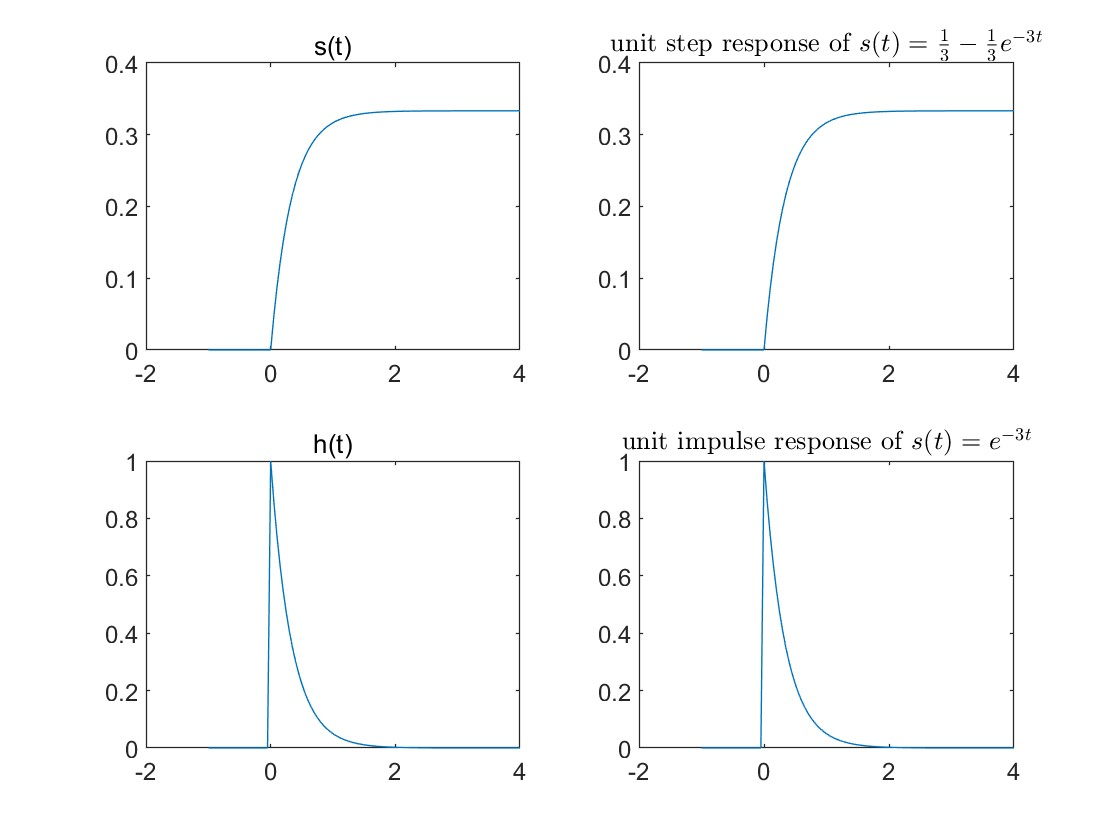
\includegraphics[width=0.75\linewidth]{figures/A2b.jpg} % 数字表示放缩比例
  \caption{Answer2b} % 图片标题
\end{figure}

\section{Problem2c,2d}
\subsection{Problem}
\begin{figure}[H]
  \centering
  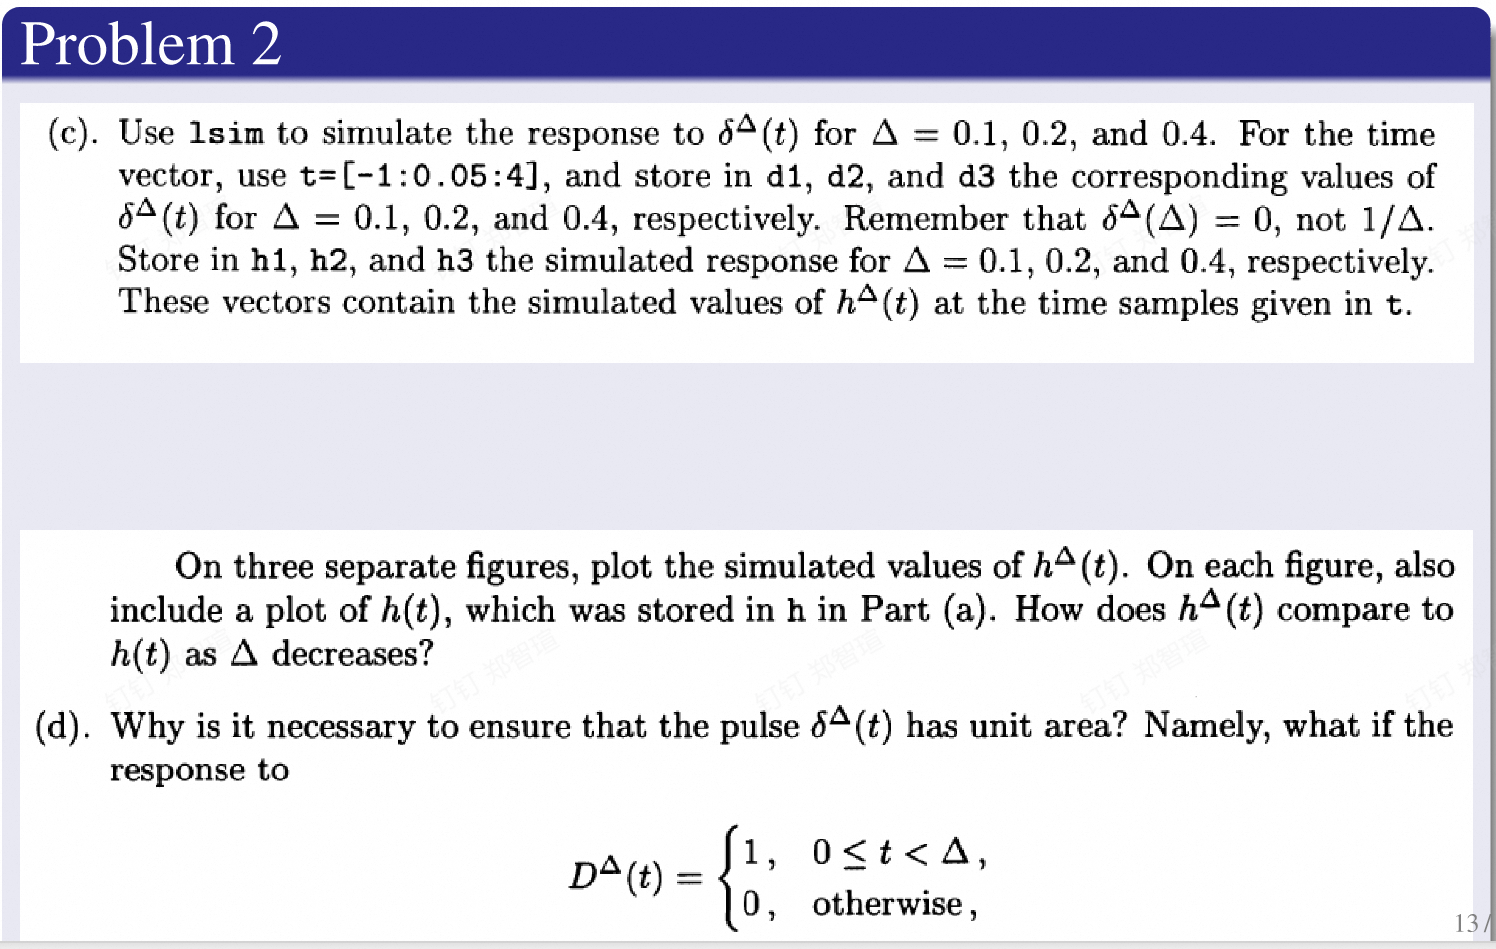
\includegraphics[width=0.75\linewidth]{figures/P22.png} % 数字表示放缩比例
  \caption{Problem2c,2d} % 图片标题
\end{figure}

\subsection{Answer}
\begin{figure}[H]
  \centering
  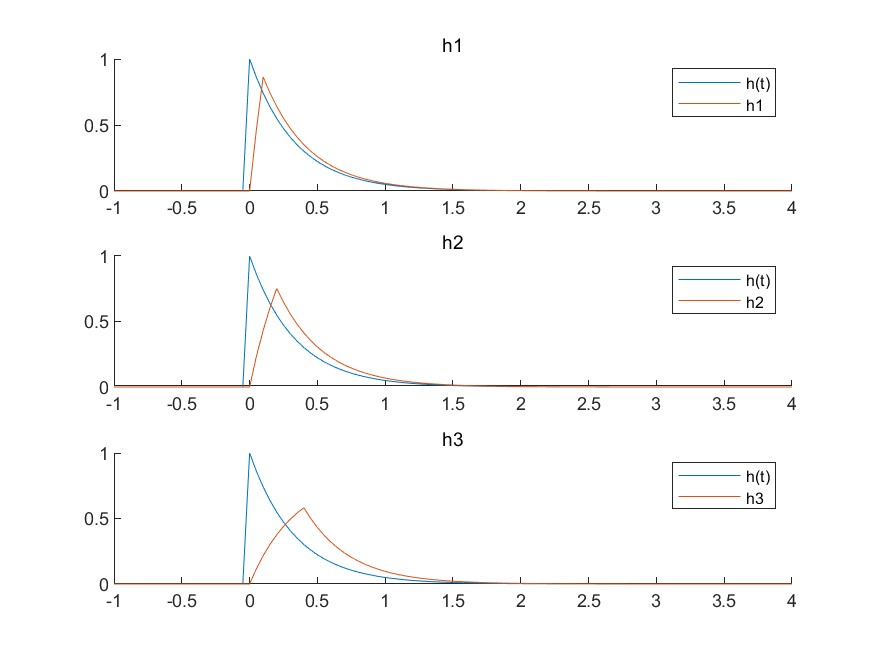
\includegraphics[width=0.75\linewidth]{figures/A2c.jpg} % 数字表示放缩比例
  \caption{Answer2c} % 图片标题
\end{figure}
Answer2d : If we directly use \( D^{\Delta}(t) \) in place of \( \delta^{\Delta}(t) \), the system's response will be scaled by \( \Delta \).
This means that if \( \Delta \) is small, the response will be underestimated, and if \( \Delta \) is large, it will be overestimated.

\section{Problem2e}
\subsection{Problem}
\begin{figure}[H]
  \centering
  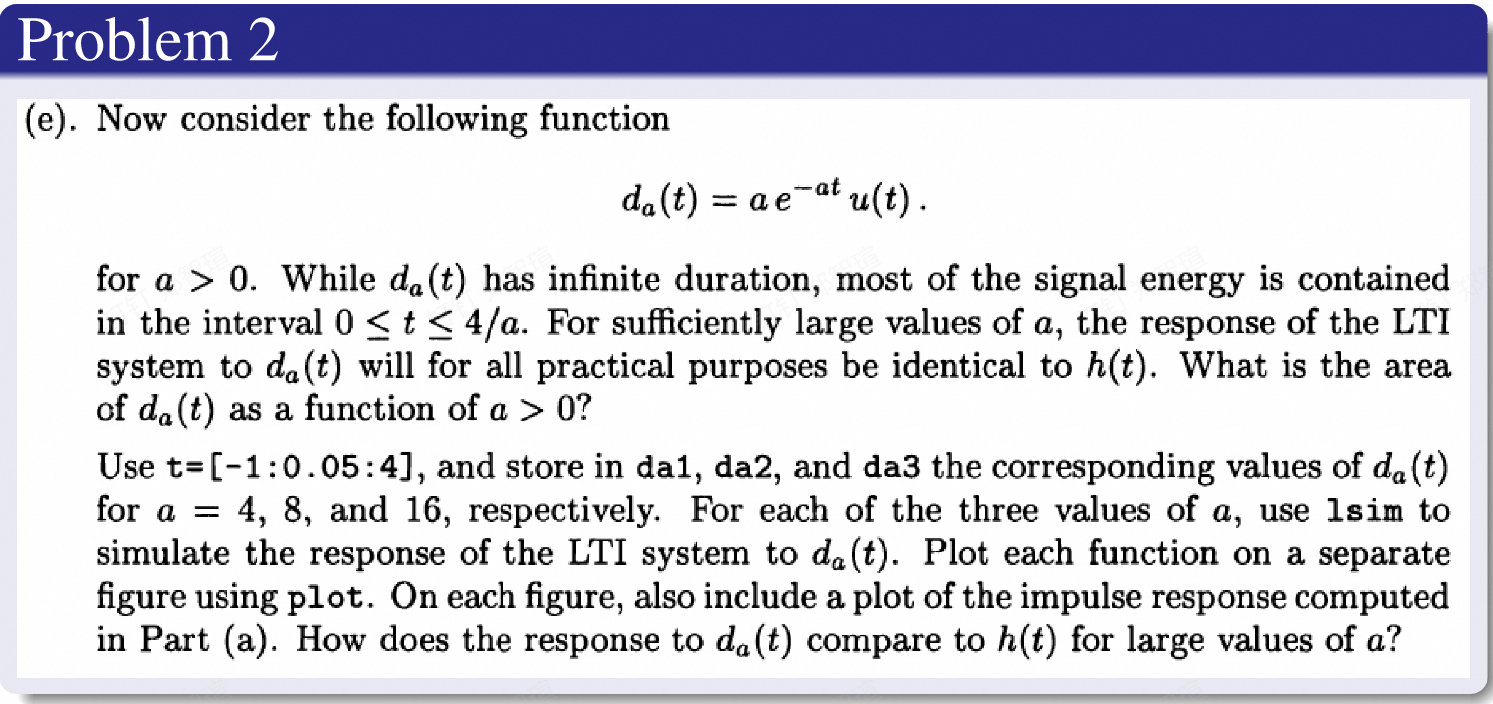
\includegraphics[width=0.75\linewidth]{figures/P23.png} % 数字表示放缩比例
  \caption{Problem2e} % 图片标题
\end{figure}
\subsection{Answer}
\begin{figure}[H]
  \centering
  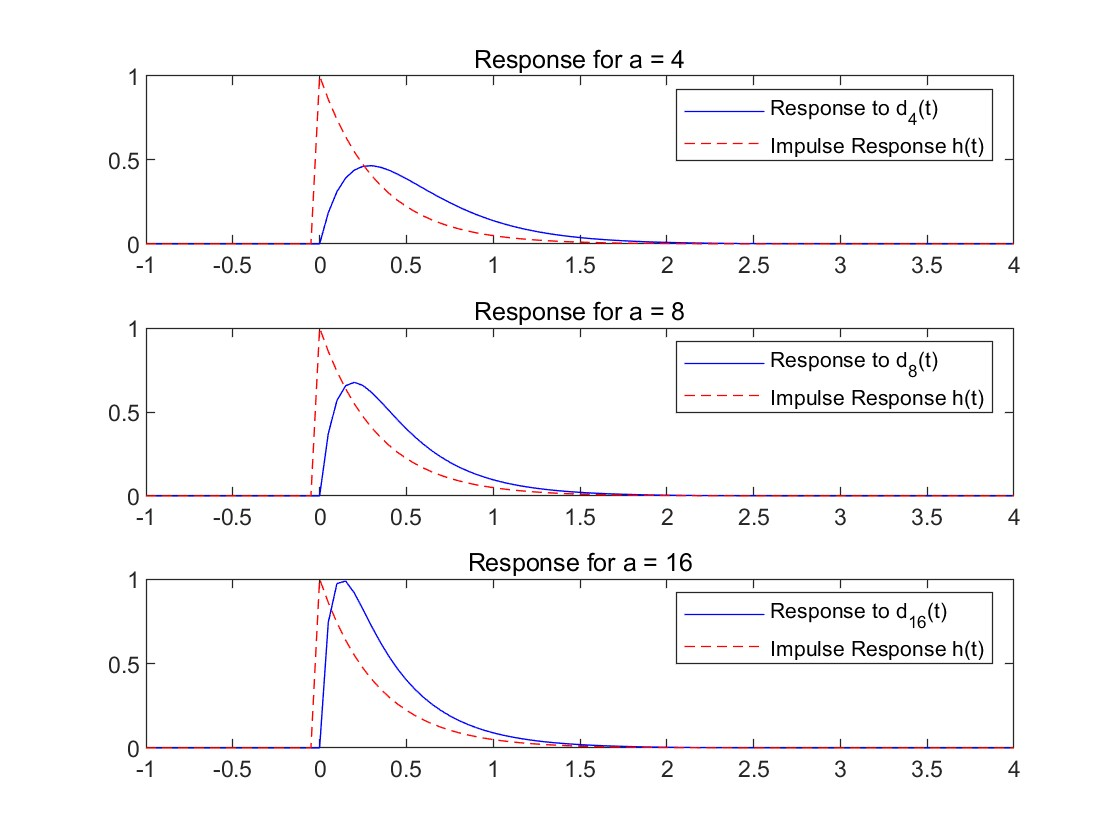
\includegraphics[width=0.75\linewidth]{figures/A2e.jpg} % 数字表示放缩比例
  \caption{Answer2e} % 图片标题
\end{figure}
For large \( a \), the response to \( d_a(t) \) approximates the impulse response \( h(t) \).
\clearpage
\section{Problem3}
\subsection{Problem}
\begin{figure}[H]
  \centering
  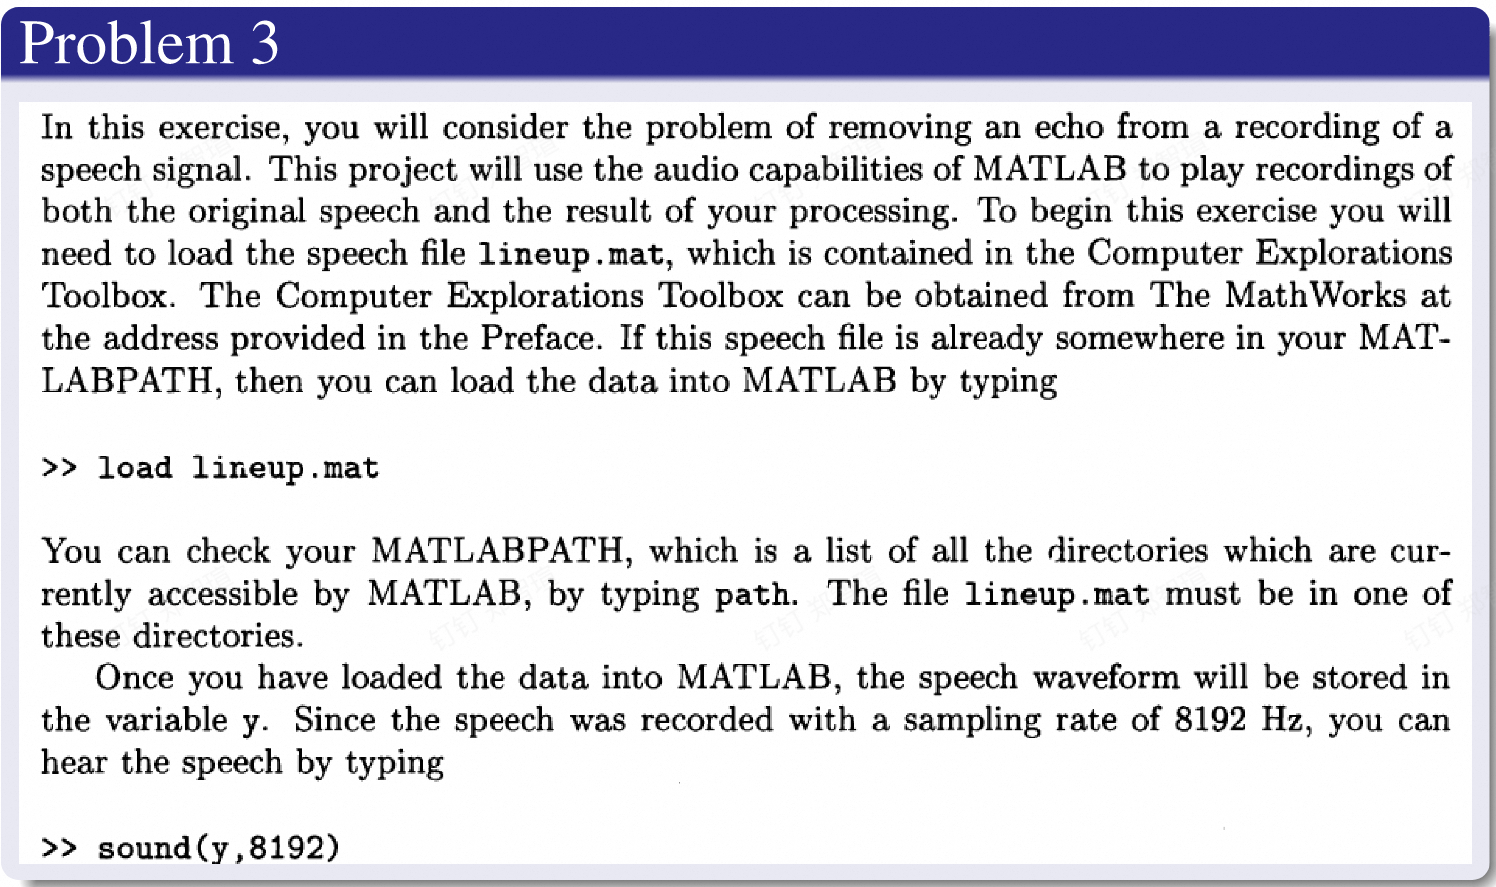
\includegraphics[width=0.75\linewidth]{figures/P31.png} % 数字表示放缩比例
  \caption{Problem3} % 图片标题
\end{figure}
\begin{figure}[H]
  \centering
  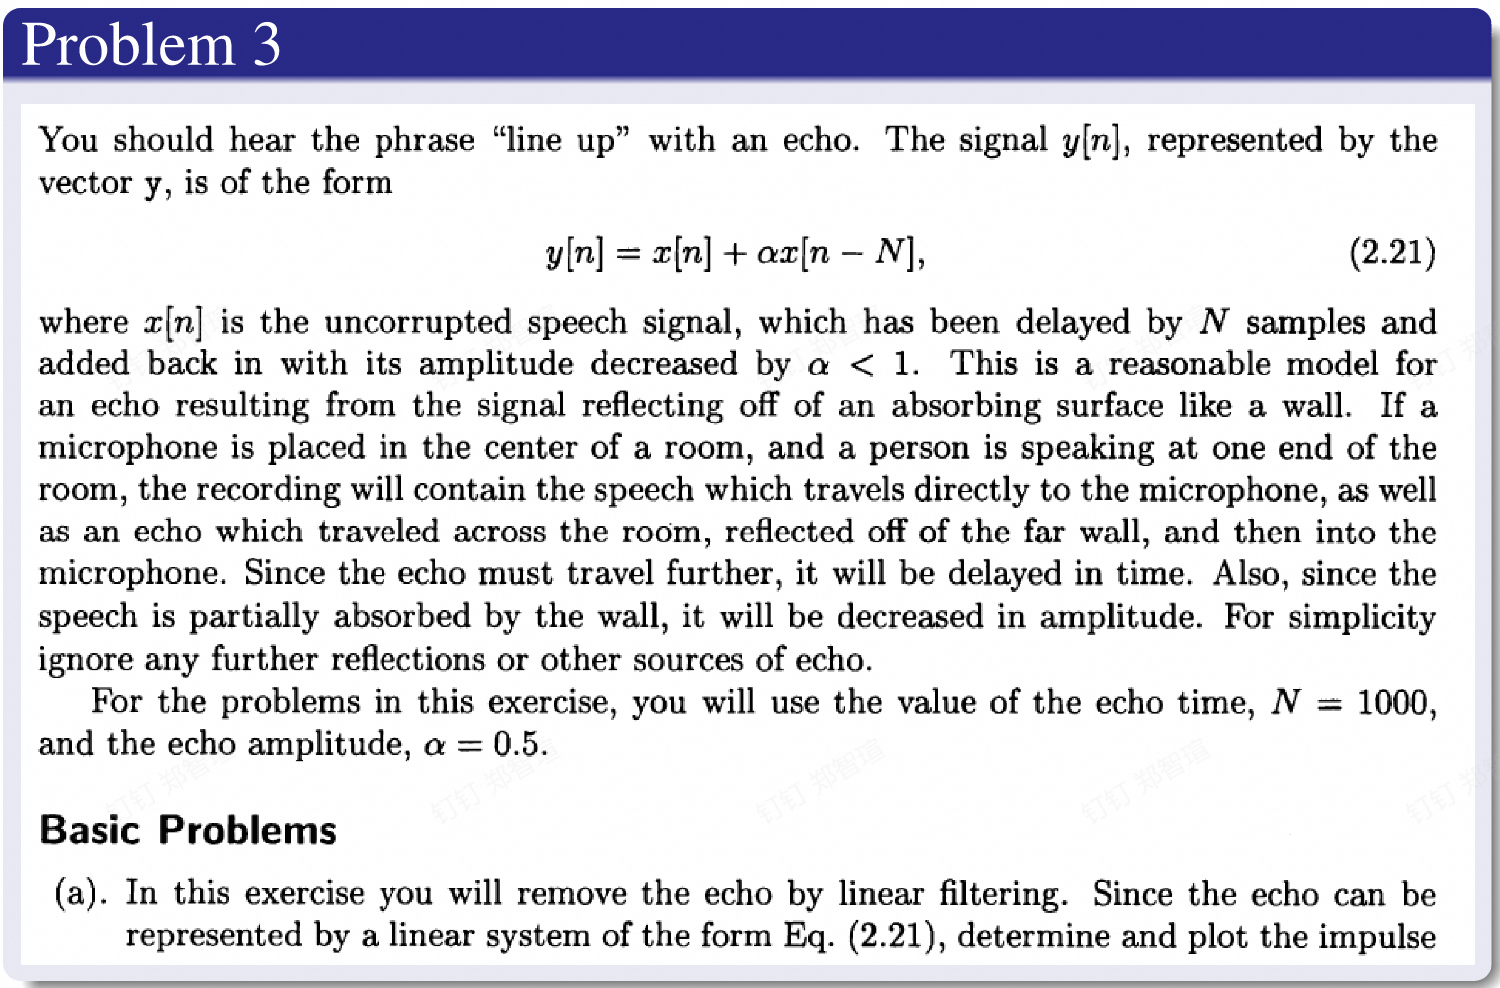
\includegraphics[width=0.75\linewidth]{figures/P32.png} % 数字表示放缩比例
  \caption{Problem3} % 图片标题
\end{figure}
\begin{figure}[H]
  \centering
  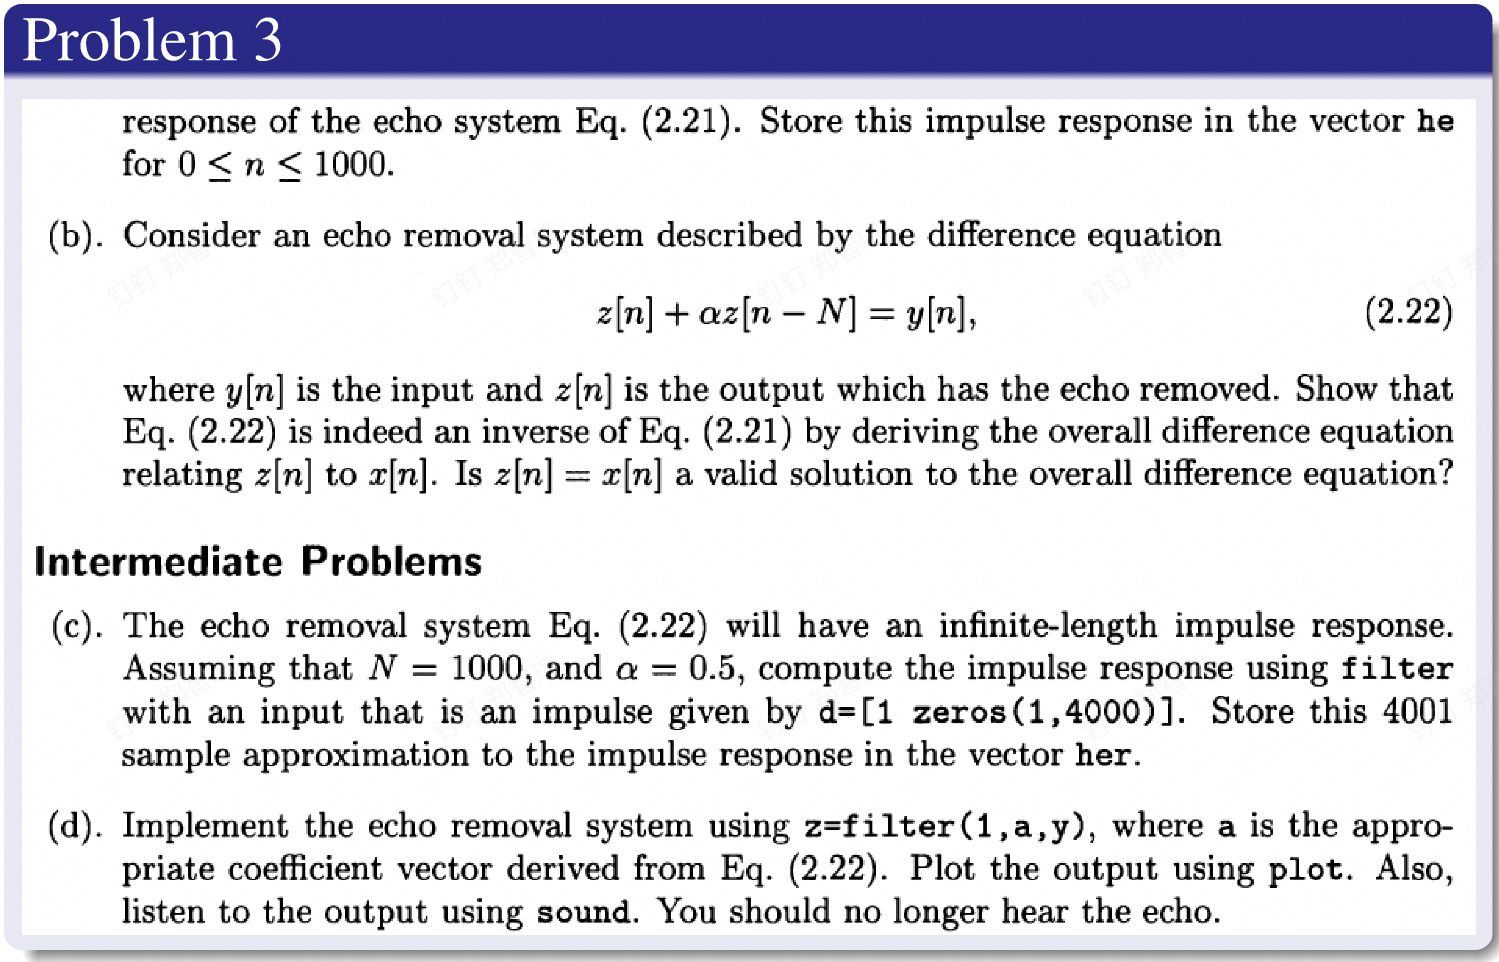
\includegraphics[width=0.75\linewidth]{figures/P33.png} % 数字表示放缩比例
  \caption{Problem3} % 图片标题
\end{figure}
\subsection{Answer}
\begin{figure}[H]
  \centering
  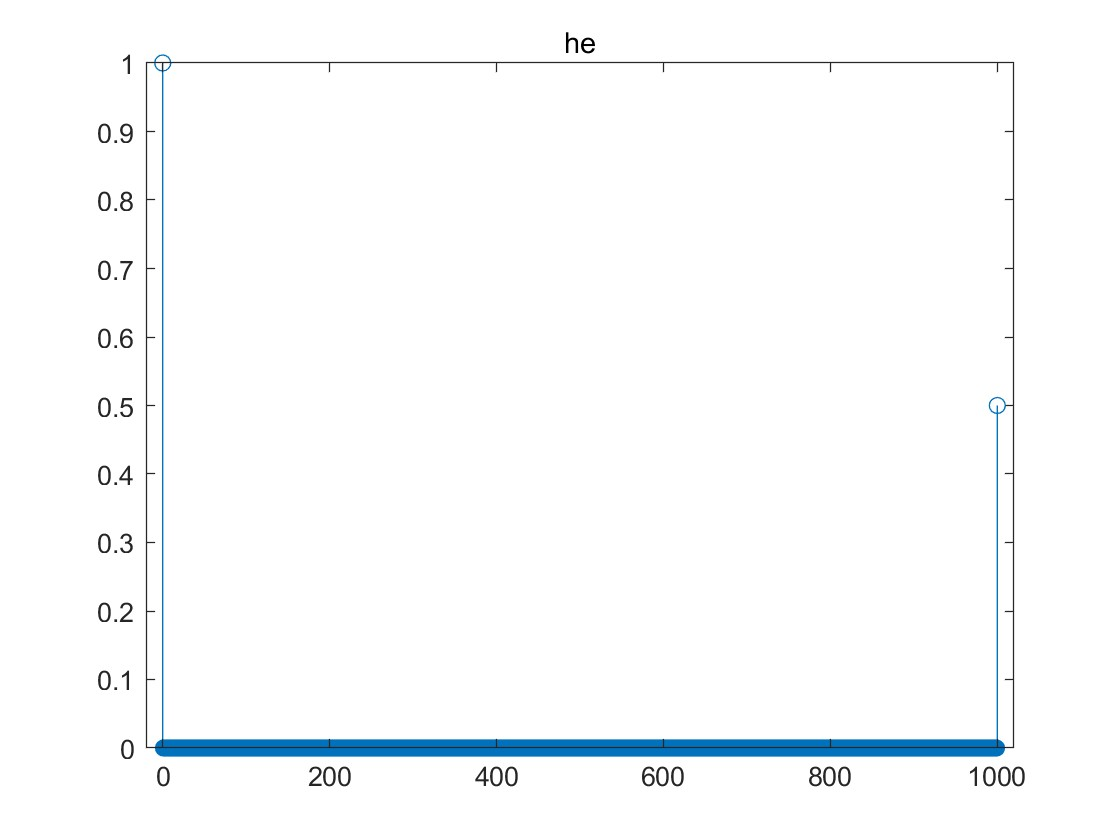
\includegraphics[width=0.75\linewidth]{figures/A3a.jpg} % 数字表示放缩比例
  \caption{Answer3a} % 图片标题
\end{figure}
Answer3b : To prove the echo removal system is the inverse, substitute \( y[n] = x[n] + \alpha x[n-N] \) into \( z[n] + \alpha z[n-N] = y[n] \). Assuming \( z[n] = x[n] \), both sides match, confirming \( z[n] = x[n] \) is valid. Thus, the system is indeed the inverse.
so \( z[n] = x[n] \) is the valid solution.
\begin{figure}[H]
  \centering
  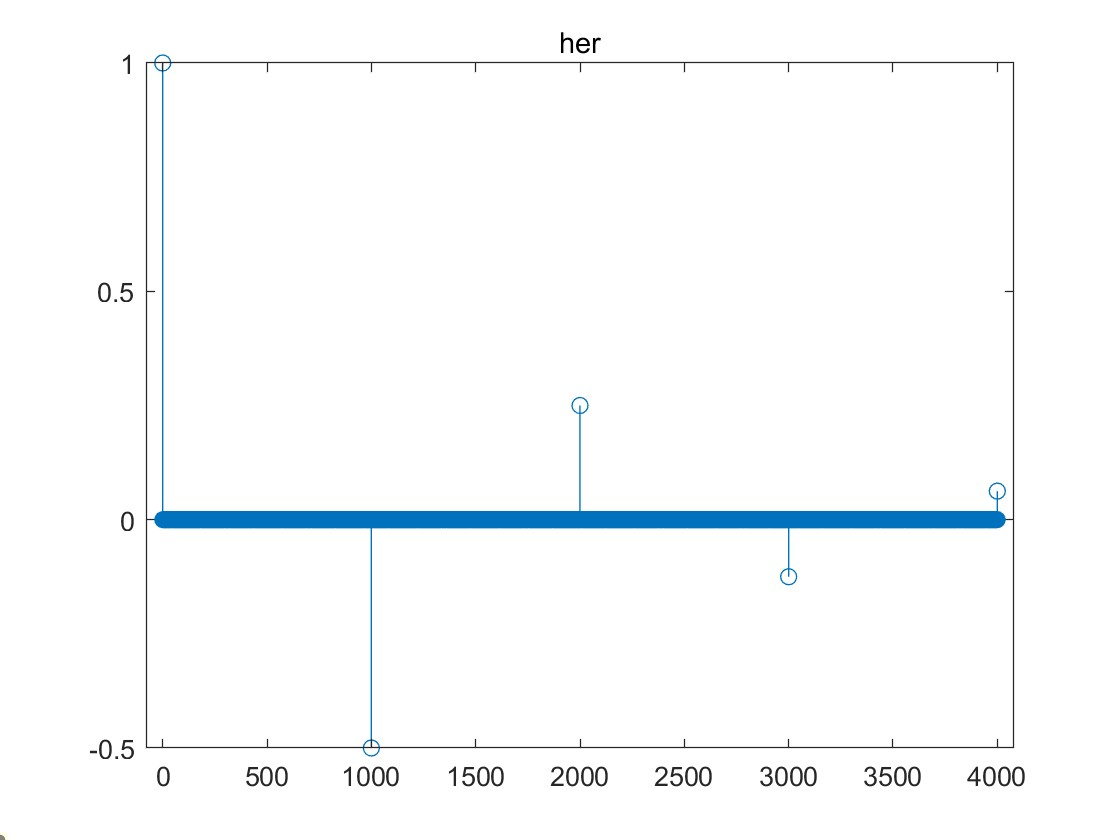
\includegraphics[width=0.75\linewidth]{figures/A3c.jpg} % 数字表示放缩比例
  \caption{Answer3c} % 图片标题
\end{figure}
\begin{figure}[H]
  \centering
  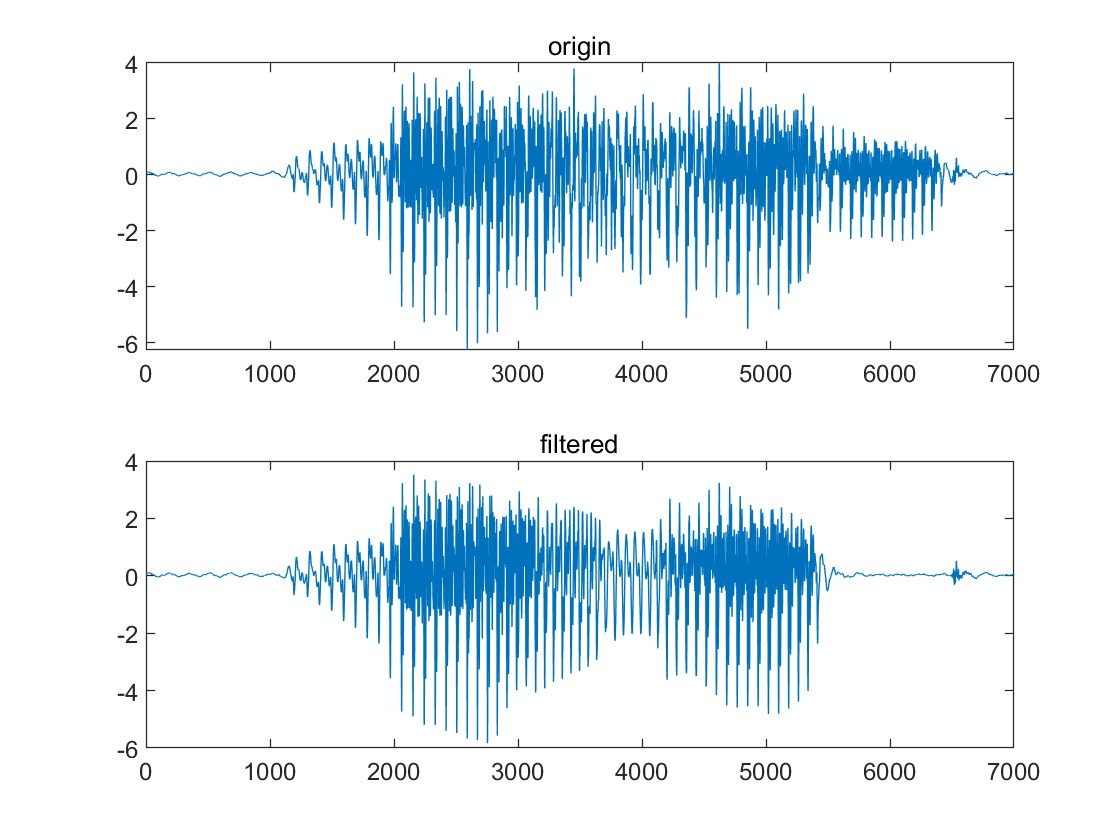
\includegraphics[width=0.75\linewidth]{figures/A3d.jpg} % 数字表示放缩比例
  \caption{Answer3d} % 图片标题
\end{figure}
\clearpage

\section{Code}
\subsection{Code1}
\begin{lstlisting}[language=matlab, caption=Problem1a Code1]
  clear;
  clc;
  
  n = 0:5;
  x1 = (n == 0);
  x2 = (n == 1);
  x3 = (n == 0) + 2*(n == 1);
  
  a=1;
  b=[1 -1 -1];
  
  w1=filter(b,a,x1);
  w2=filter(b,a,x2);
  w3=filter(b,a,x3);
  w4=w1+2*w2;
  
  subplot(4,1,1);
  stem(n,w1);
  title("w1");
  
  subplot(4,1,2);
  stem(n,w2);
  title("w2");
  
  subplot(4,1,3);
  stem(n,w3);
  title("w3");
  
  subplot(4,1,4);
  stem(n,w4);
  title("w1+2*w2");
  
  sgtitle("\omega [n]=x[n]-x[n-1]-x[n-2]");
\end{lstlisting}
\clearpage
\begin{lstlisting}[language=matlab, caption=Problem1a Code2]
  clear;
  clc;

  n=0:5;
  x1=[1 0 0 0 0 0];
  x2=[0 1 0 0 0 0];
  x3=x1+2*x2;

  w1=cos(x1);
  w2=cos(x2);
  w3=cos(x3);
  w4=w1+2*w2;


  subplot(4,1,1);
  stem(n,w1);
  title('y1');

  subplot(4,1,2);
  stem(n,w2);
  title('y2');

  subplot(4,1,3);
  stem(n,w3);
  title('y3');

  subplot(4,1,4);
  stem(n,w4);
  title('y1+2*y2');

  sgtitle("y[n]=cos(x[n])");
\end{lstlisting}
\clearpage
\begin{lstlisting}[language=matlab, caption=Problem1a Code3]
  clear;
  clc;

  n=0:5;
  x1=[1 0 0 0 0 0];
  x2=[0 1 0 0 0 0];
  x3=x1+2*x2;

  w1=n.*x1;
  w2=n.*x2;
  w3=n.*x3;
  w4=w1+2*w2;


  subplot(4,1,1);
  stem(n,w1);
  title('z1');

  subplot(4,1,2);
  stem(n,w2);
  title('z2');

  subplot(4,1,3);
  stem(n,w3);
  title('z3');

  subplot(4,1,4);
  stem(n,w4);
  title('z1+2*z2');

  sgtitle("z[n]=nx[n]");
\end{lstlisting}
\clearpage
\subsection{Code2}
\begin{lstlisting}[language=matlab, caption=Problem2b Code]
  clear;
  clc;
  
  t=-1:0.05:4;
  t_=0:0.05:4;
  u=[zeros(1,length(-1:0.05:-0.05)) ones(1,length(0:0.05:4))];
  
  s=(1/3-1/3*exp(-3*t)).*u;
  h=exp(-3*t).*u;
  
  a=[1 3];
  b=1;
  
  s1=step(b,a,t_);
  s1=[zeros(1,length(-1:0.05:-0.05)) s1.'];
  
  h1=impulse(b,a,t_);
  h1=[zeros(1,length(-1:0.05:-0.05)) h1.'];
  
  subplot(2,2,2);
  plot(t,s);
  title('$\frac{1}{3} - \frac{1}{3} e^{-3t}$', 'Interpreter', 'latex')
  
  subplot(2,2,1);
  plot(t,s1);
  title('s(t)');
  
  subplot(2,2,4);
  plot(t,h);
  title('$e^{-3t}$', 'Interpreter', 'latex')
  
  subplot(2,2,3);
  plot(t,h1);
  title('h(t)');
\end{lstlisting}
\begin{lstlisting}[language=matlab, caption=Problem2c Code]
  clear;
  clc;

  t=-1:0.05:4;
  t_=0:0.05:4;

  delta1=0.1;
  delta2=0.2;
  delta3=0.4;

  d1=[zeros(1,length(-1:0.05:-0.05)) ones(1,length(0:0.05:delta1-0.05))/delta1 zeros(1,length(delta1:0.05:4))];
  d2=[zeros(1,length(-1:0.05:-0.05)) ones(1,length(0:0.05:delta2-0.05))/delta2 zeros(1,length(delta2:0.05:4))];
  d3=[zeros(1,length(-1:0.05:-0.05)) ones(1,length(0:0.05:delta3-0.05))/delta3 zeros(1,length(delta3:0.05:4))];

  a=[1 3];
  b=1;
  h1=lsim(b,a,d1,t);
  h2=lsim(b,a,d2,t);
  h3=lsim(b,a,d3,t);
  h=impulse(b,a,t_);
  h=[zeros(1,length(-1:0.05:-0.05)) h.'];

  subplot(3,1,1);
  hold on;
  p1 = plot(t,h, 'DisplayName', 'h(t)');
  p2 = plot(t,h1, 'DisplayName', 'h1');
  title('h1');
  legend([p1, p2]);

  subplot(3,1,2);
  hold on;
  p1 = plot(t,h, 'DisplayName', 'h(t)');
  p2 = plot(t,h2, 'DisplayName', 'h2');
  title('h2');
  legend([p1, p2]);

  subplot(3,1,3);
  hold on;
  p1 = plot(t,h, 'DisplayName', 'h(t)');
  p2 = plot(t,h3, 'DisplayName', 'h3');
  title('h3');
  legend([p1, p2]);

\end{lstlisting}
\begin{lstlisting}[language=matlab, caption=Problem2e Code]
  clear;
  clc;

  t=-1:0.05:4;

  a1 = 4; a2 = 8; a3 = 16;
  da1 = a1 * exp(-a1 * t) .* (t >= 0);
  da2 = a2 * exp(-a2 * t) .* (t >= 0);
  da3 = a3 * exp(-a3 * t) .* (t >= 0);

  h = exp(-3 * t) .* (t >= 0);

  a=[1 3];
  b=1;
  y1 = lsim(b, a, da1, t);
  y2 = lsim(b, a, da2, t);
  y3 = lsim(b, a, da3, t);

  subplot(3,1,1);
  plot(t, y1, 'b', t, h, 'r--');
  legend('Response to d_4(t)', 'Impulse Response h(t)');
  title('Response for a = 4');

  subplot(3,1,2);
  plot(t, y2, 'b', t, h, 'r--');
  legend('Response to d_8(t)', 'Impulse Response h(t)');
  title('Response for a = 8');

  subplot(3,1,3);
  plot(t, y3, 'b', t, h, 'r--');
  legend('Response to d_{16}(t)', 'Impulse Response h(t)');
  title('Response for a = 16');
\end{lstlisting}
\clearpage
\subsection{Code3}
\begin{lstlisting}[language=matlab, caption=Problem3a Code]
  clear;
  clc;
  
  alpha=0.5;
  N=1000;
  n=0:1000;
  
  he = [1 zeros(1,N-1) alpha];
  
  stem(n,he);
  title("he");
\end{lstlisting}
\begin{lstlisting}[language=matlab, caption=Problem3c Code]
  clear;
  clc;
  
  n = 0:4000;
  N = 1000;
  alpha = 0.5;
  a = [1, zeros(1, N-1), alpha];
  d = [1, zeros(1, 4000)];
  her = filter(1, a, d);
  stem(n,her);
  title('her');
\end{lstlisting}
\clearpage
\begin{lstlisting}[language=matlab, caption=Problem3d Code]
  clear;
  clc;
  
  load lineup.mat
  
  alpha=0.5;
  n=0:1:7000;
  N=1000;
  
  a=1;
  b=[1 zeros(1,N-1) alpha];
  
  y_ = filter(a,b,y);
  sound(y ,8192);
  pause(2);
  sound(y_ ,8192);
  
  subplot(2,1,1)
  plot(y);
  title('origin');
  
  subplot(2,1,2)
  plot(y_);
  title('filtered')
\end{lstlisting}
\end{document}
